\documentclass{article}
\usepackage{algpseudocode}
\usepackage[ruled]{algorithm}
\usepackage{url}
\usepackage{framed}
\usepackage{amsfonts,amsmath,amsthm,amssymb}
\usepackage{graphicx}
\usepackage{url}
\usepackage{color}
\usepackage{geometry}

\geometry{margin=1.2in}

\newcommand {\mean} {\ensuremath {\mathop{\mathrm{mean}}}}
\newcommand {\median} {\ensuremath {\mathop{\mathrm{median}}}}
\newcommand {\N} {\ensuremath {\mathcal{N}}}
\newcommand {\IE} {\ensuremath {\mathbb{E}}}
\newcommand {\cov} {\ensuremath {\mathop{\mathrm{cov}}}}
\newcommand {\BEL} {\ensuremath {\mathop{\mathrm{BEL}}}}

\newtheorem{lemma}{Lemma}

\title{Doing Better Than UCT: \\ Rational Monte Carlo Sampling in Trees}
\author {David Tolpin, Solomon Eyal Shimony \\
Department of Computer Science, \\
Ben-Gurion University of the Negev, Beer Sheva, Israel \\
\{tolpin,shimony\}@cs.bgu.ac.il}

\begin{document}

\maketitle

\begin{abstract}
UCT, a state-of-the art algorithm for Monte Carlo tree sampling
(MCTS), is based on UCB, a sampling policy for the Multi-armed Bandit
Problem (MAB) that minimizes the accumulated regret. However, MCTS
differs from MAB in that only the final choice, rather than all arm
pulls, brings a reward, that is, the simple regret, as opposite to the
cumulative regret, must be minimized. This work introduces policies for
multi-armed bandits with lower simple regret than UCB, and an
algorithm for MCTS which combines cumulative and simple regret
minization and outperforms UCT. Finite-time and asymptotic analysis of
the policies is provided, and the algorithms are empirically compared.
\end{abstract}

\section{Introduction and definitions}

The Multi-armed Bandit is a set of $K$ arms. Each arm can be pulled
multiple times. When the $i$th arm is pulled, a random reward $X_i$
from an unknown stationary distribution is returned.  The reward is 
bounded between 0 and 1. 

The simple regret of a sampling policy for the Multi-armed Bandit
Problem is the expected difference between the best expected reward
$\mu_*$ and the expected reward $\mu_j$ of the arm with the best sample mean
$\overline X_j=\max_i\overline X_i$:
\begin{equation}
\label{eq:simple-regret}
\IE[R]=\sum_{j=1}^K\Delta_j\Pr(\overline X_j=\max_i\overline X_i)
\end{equation}
where $\Delta_j=\mu_*-\mu_j$.
Strategies that minimize the simple reward are called pure exploration
strategies \cite{Bubeck.pure}.

Such strategies are used to select the best arm, and, by extension,
the best action in Monte Carlo tree search. Monte Carlo tree search is
used to solve Markov Decision Processes (MDP) approximately. An MDP is
defined by the set of states $S$, the set of actions $A$, the
transition table $T(s, a, s')$, the reward table $R(s, a, s')$, the
initial state $s$ and the goal state $t$: $(S, A, T, R, s, t)$
\cite{Russell.aima}.  Monte Carlo tree search explores an MDP by
\emph{rollouts}---trajectories from the current state to a state in
which a termination condition is satisfied (either the goal state, or
a cutoff state for which the reward is evaluated
approximately). Algorithm UCB that minimizes the cumulative regret
\cite{Auer.ucb} had been extended to tree search as UCT
\cite{Kocsis.uct}.

UCT-driven search achieves good results in many search problems. At each
search step, the algorithm allocates Monte Carlo rollouts to choose
the best action, thereby minimizing the cumulative regret. However, the
simple and the cumulative regret cannot be minimized simultaneously;
moreover, \cite{Bubeck.pure} shows that in many cases the smaller the
cumulative regret, the greater the simple regret.

UCT performance can be improved by combining UCB with a sampling
scheme that minimizes the simple regret of selecting an action at the
current root node. Indeed, the algorithm must select an action with
the minimum regret \emph{given the assumption that after performing the selected action
the algorithm performs optimally}, which corresponds to maximizing the
value of partial information \cite{Russell.aima}. Therefore, an
improved allocation scheme would
\begin{itemize}
\item maximize the value of partial
information by sampling actions to minimize the \textbf{simple} regret at the
current root node, and then 
\item minimize the \textbf{cumulative} regret of the rollouts from the second
  step on to approach the optimum behavior. 
\end{itemize}


\section{Main Results}

\subsection{Doing better than UCB}

\begin{enumerate}
\item The $\varepsilon$-greedy allocation scheme has exponential convergence
rate of the simple regret $\IE r$ (see Appendix~\ref{app:derivations-finite-eps}):
\begin{equation}
  \IE r_\varepsilon\le\sum_{j=1}^K\Delta_j\left(\frac {n\varepsilon} K + \frac {4\sqrt e}
{\Delta_j^2}\right)e^{-\Delta_j^2n\varepsilon/8K}
\end{equation}
\item The UCB allocation scheme exhibits polynomial convergence
rate (see Appendix~\ref{app:derivations-finite-ucb}):
\begin{equation}
\IE r_{ucb} \le 2\sum_{j=1}^K \Delta_jn^{\frac {-\alpha \Delta_j^2} 8}
\end{equation}
\item A tighter upper regret bound for the $\varepsilon$-greedy allocation scheme depends on
$\varepsilon$. The lowest bound is
acheived for $\varepsilon=\frac 1
2$, and for a large number of arms the bound for the $\frac 1 2$-greedy scheme approaches the square of the
bound for uniform sampling (see
Appendix~\ref{app:derivations-asym-eps}).
\end{enumerate}

Another improved allocation scheme for minimizing the simple regret,
called \textbf{UQB} here, is obtained by substituting $\sqrt{\cdot}$
instead of $\log(\cdot)$ into the formula for UCB and has a
superpolynomial convergence rate (see
Appendix~\ref{app:derivations-asym-ucb}).

\subsection{Doing better than UCT}

The {\bf two-stage} Monte Carlo tree search sampling
scheme selects an action at the current root node according to an
algorithm that minimizes the simple regret, such as $\frac 1 2$-greedy or
UQB, and then selects actions according to UCB. Such two-stage
outperforms the UCT sampling scheme that selects actions based on
UCB only.

Such sampling scheme is significantly less sensitive to the tuning of
the exploration factor ($C_p$ in \cite{Kocsis.uct}) of UCT, since the
conflict \cite{Bubeck.pure} between the need for a larger value of
$C_p$ on the first step (simple regret) and a smaller value for the
rest of the rollout (cumulative regret) is resolved. In fact, a
sampling scheme that uses UCB at all steps but a larger value of $C_p$
for the first step than for the rest of the steps, outperforms
UCT. The pseudocode of the two-stage rollout is in
Algorithm~\ref{alg:two-stage-mcts}.

\begin{algorithm}[t]
\caption{Two-stage Monte-Carlo tree search sampling}
\label{alg:two-stage-mcts}
\begin{algorithmic}[1]
\Procedure{Rollout}{node, depth=1}
  \If {\Call{IsLeaf}{node, depth}}
    \State \textbf{return} 0
  \Else
    \If {depth=1}
      \State action $\gets$ \Call{FirstAction}{node} \Comment minimizes simple regret, e.g. $\frac 1 2$-greedy
    \Else
      \State action $\gets$ \Call{NextAction}{node} \Comment  UCB --- minimizes cumulative regret
    \EndIf
    \State next-node $\gets$ \Call{NextState}{node, action}
    \State reward $\gets$ \Call{TransitionReward}{node, action, next-node}
    \State \hspace{4em} + \Call{Rollout}{next-node, depth+1} \Comment call {\sc Rollout} recursively
    \State \Call{UpdateStats}{node, action, reward}
  \EndIf
\EndProcedure
\end{algorithmic}
\end{algorithm}

\section{Empirical Evaluation}

The results were empirically verified on Multi-armed Bandit instances
(Section~\ref{seq:emp-mab}), on search trees
(Section~\ref{seq:emp-mcts}), and on the sailing domain
(Section~\ref{seq:emp-sailing}), as defined in \cite{Kocsis.uct}. The
experiments confirmed the hypotheses. The algorithms used in the
experiments are:
\begin{description}
\item[RND:] uniform \underline{r}a\underline{nd}om samping;
\item[UCT:] \underline{U}pper \underline{C}onfidence Bounds applied to
  \underline{T}rees \cite{Kocsis.uct};
\item[GCT:] U\underline{CT} with the first step
  replaced with $\frac 1 2$-\underline{g}reedy sampling;
\item[QCT:] U\underline{CT} with the first step
  replaced with U\underline{Q}B.
\end{description}

\subsection{Simple regret in multi-armed bandits}
\label{seq:emp-mab}

Figure~\ref{fig:mab-simple-regret} presents a comparison of simple
regret minimization algorithms for Multi-armed
bandits. Figure~\ref{fig:mab-simple-regret}.a shows the search tree
corresponding to a problem instance. Each arm returns a random reward
drawn from a Bernoulli distribution. The search selects an arm
and compares the expected reward, unknown to the algorithm during the
sampling, to the expected reward of the best arm.

Figure~\ref{fig:mab-simple-regret}.b shows the regret
vs. the number of samples, averaged
over $10^4$ experiments for randomly generated instances of 32 arms. 

For smaller numbers of samples, $\frac 1 2$-greedy achieves the best
performance; for large number of samples, QCT outperforms GCT. QCT is
better than UCT everywhere except for very small numbers of samples. A
combination of GCT and QCT dominates UCT over the whole range.

\begin{figure}[t]
  \begin{minipage}[c]{0.5\linewidth}
    \centering
    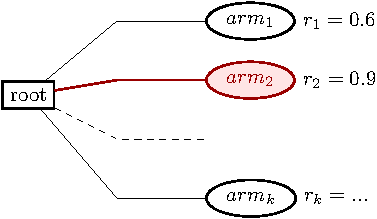
\includegraphics[scale=1.0]{onelevel-tree.pdf}\\
    \vspace{4em}
    a. search tree
  \end{minipage}
  \begin{minipage}[c]{0.5\linewidth}
    \centering
    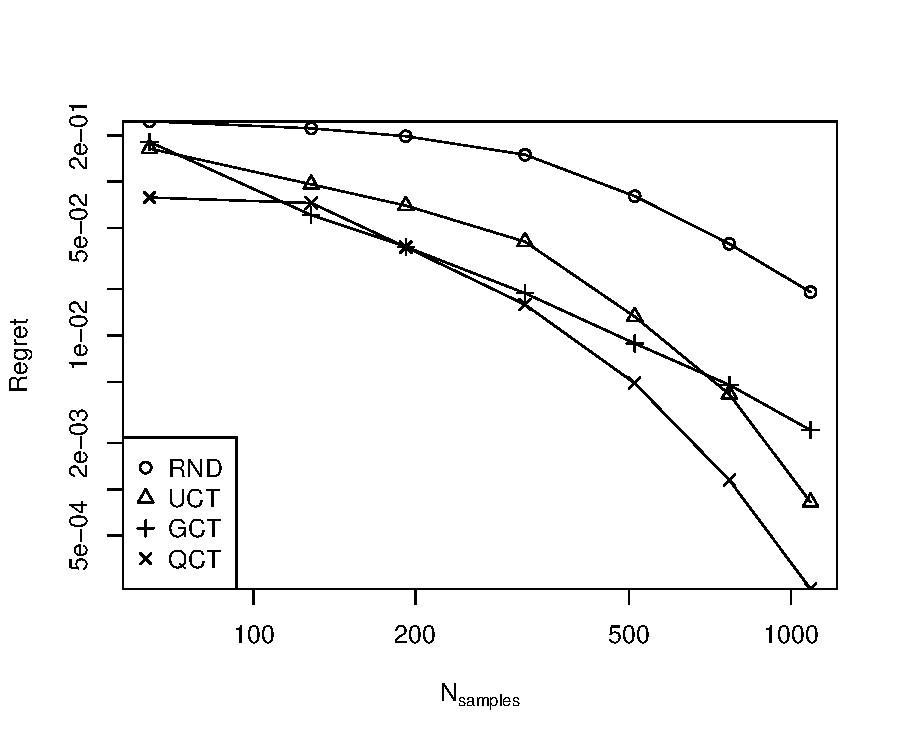
\includegraphics[scale=0.5]{flat-trilevel-k=64-uqb=8.pdf}\\
    b. regret vs. number of samples
  \end{minipage}
  \label{fig:mab-simple-regret}
  \caption{Simple regret in MAB}
\end{figure}

\subsection{Monte Carlo tree search}
\label{seq:emp-mcts}

The second set of experiments was performed on randomly generated
trees crafted in such a way that uniform random sampling selects a
direction at the root randomly. The degree of the root is a parameter of
the tree generator. The degree of all nodes at distance 1 from the
root is 2, and all nodes at distance 2 from the roots are leaves. The
average reward of two children of each node at distance 1 is
0.5. Thus, a uniform sampling scheme results in the same average reward for
all edges at the root, and an adaptive sampling scheme, such as UCT,
has to be used.

Figure~\ref{fig:mcts-regret} shows a sketch of the search tree
(Figure~\ref{fig:mcts-regret}.a) and the dependency of the regret vs. the
number of samples for trees with root degree 16
(Figure~\ref{fig:mcts-regret}.b) and 64 (Figure~\ref{fig:mcts-regret}.c). The
dependencies look differently from Multi-armed bandit instances, but
the algorithms exhibit a similar relative performance: either GCT or QCT
is always better than UCT, QCT dominates UCT everywhere
except for small numbers of instances. The advantage of QCT grows with
the number of arms.

\begin{figure}
  \begin{minipage}[c]{0.5\linewidth}
    \centering
    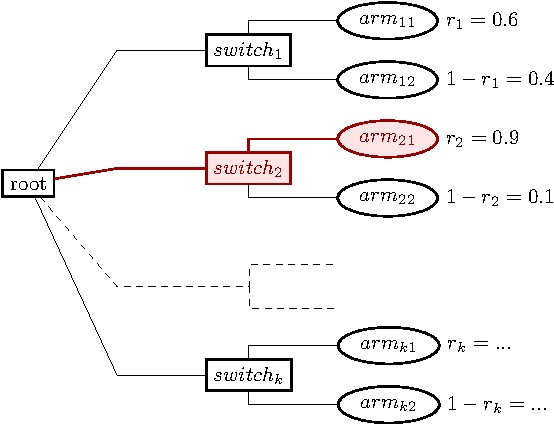
\includegraphics[scale=0.8]{twolevel-tree.pdf}\\
    a. search tree
  \end{minipage}
  \begin{minipage}[c]{0.5\linewidth}
    \centering
    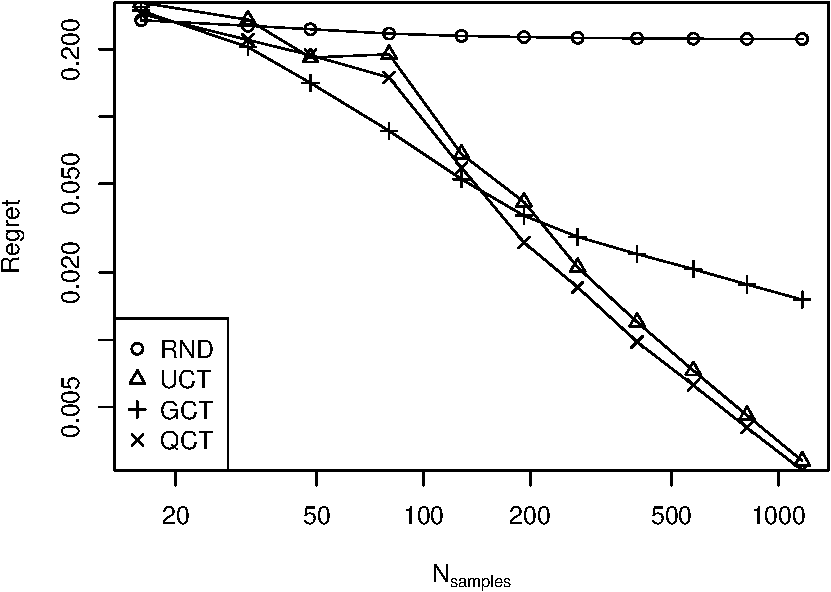
\includegraphics[scale=0.4]{tree-identity-k=16-uqb=8.pdf}\\ 
    b. 16 arms \\
    \vspace{1em}
    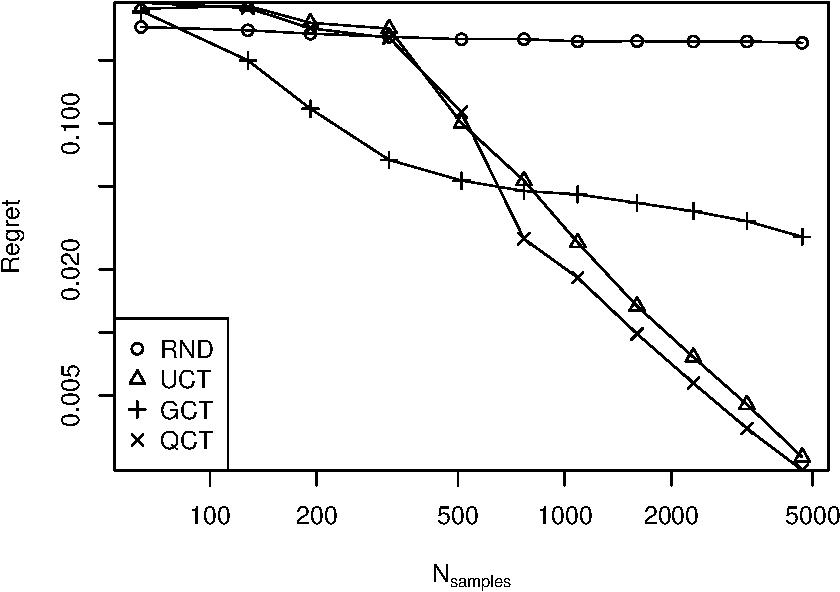
\includegraphics[scale=0.4]{tree-identity-k=64-uqb=8.pdf} \\
    c. 64 arms
 \end{minipage}
  \label{fig:mcts-regret}
  \caption{MCTS: a path to the best arm}
\end{figure}

\subsection{The sailing domain}
\label{seq:emp-sailing}

Figures~\ref{fig:sailing-cost-vs-nsamples}--\ref{fig:sailing-rcq-vs-factor}
show results of experiments on the sailing
domain. Figure~\ref{fig:sailing-cost-vs-nsamples} shows the regret
vs. the number of samples, computed for a range of values of
$C_p$. Figure~\ref{fig:sailing-cost-vs-nsamples}.a shows the median
cost, and Figure~\ref{fig:sailing-cost-vs-nsamples}.b --- the minimum
costs. UCT is always worse than either $\frac 1 2$-greedy (GCT) or QCT, and is sensitive to
the value of $C_p$: the median cost is much higher than the minimum
cost for UCT. For both $\frac 1 2$-greedy and QCT, the difference is
significantly less prominent.

\begin{figure}[t]
  \begin{minipage}[b]{0.5\linewidth}
    \centering
    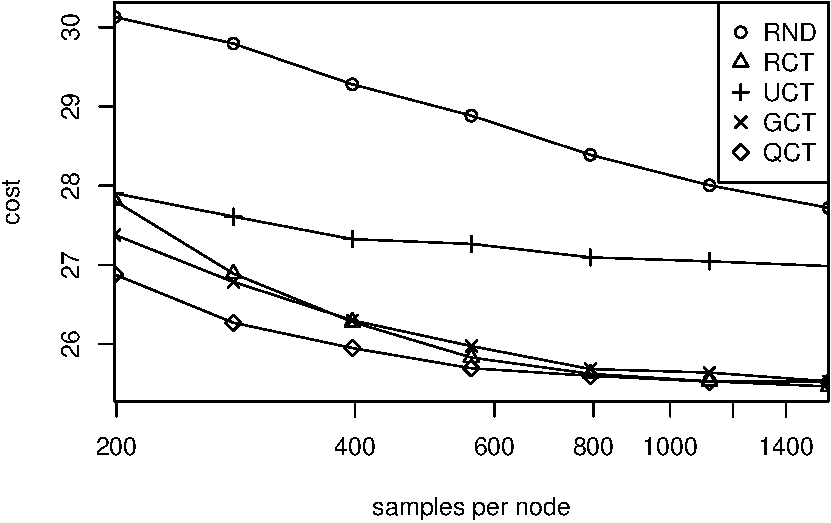
\includegraphics[scale=0.45]{costs-size=6-group=median.pdf}\\
    a. median cost
  \end{minipage}
  \begin{minipage}[b]{0.5\linewidth}
    \centering
    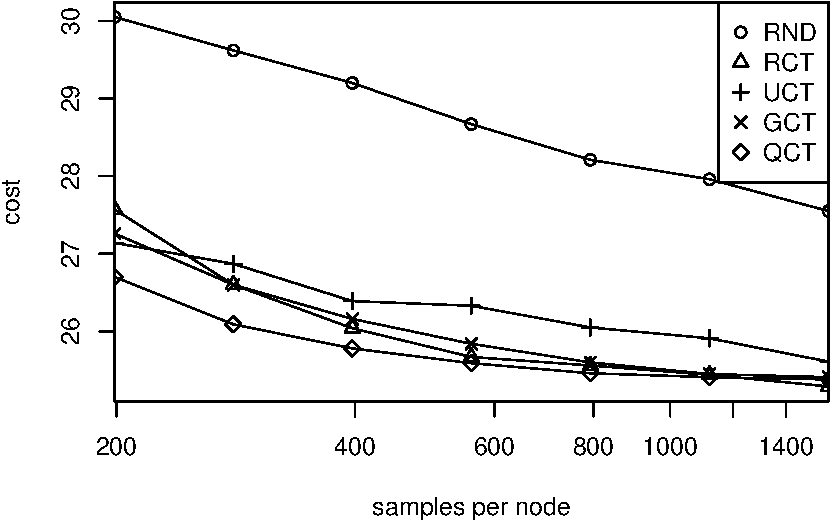
\includegraphics[scale=0.45]{costs-size=6-group=minimum.pdf}\\
    b. minimum cost
  \end{minipage}
  \caption{The sailing domain, $6\times 6$ lake, cost vs. number of rollouts}
  \label{fig:sailing-cost-vs-nsamples}
\end{figure}

Figure~\ref{fig:sailing-cost-vs-factor} shows the rerget vs. the
exploration factor for different numbers of samples. QCT is always better than
UCT, and $\frac 1 2$-greedy is better than UCT expect for a small range of
values of the exploration factor $C_p$. 

\begin{figure}[t]
  \begin{minipage}[b]{0.5\linewidth}
    \centering
    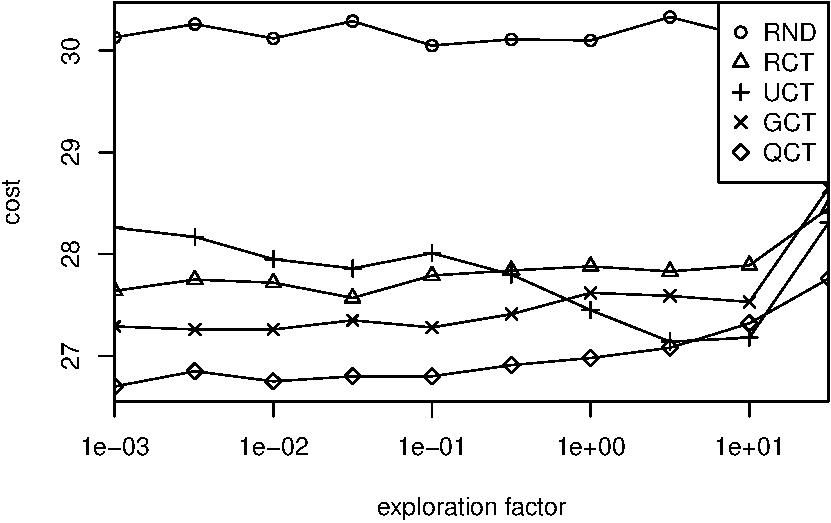
\includegraphics[scale=0.45]{costs-size=6-nsamples=199.pdf}\\
    a. 199 rollouts\\
    \vspace{1em}
    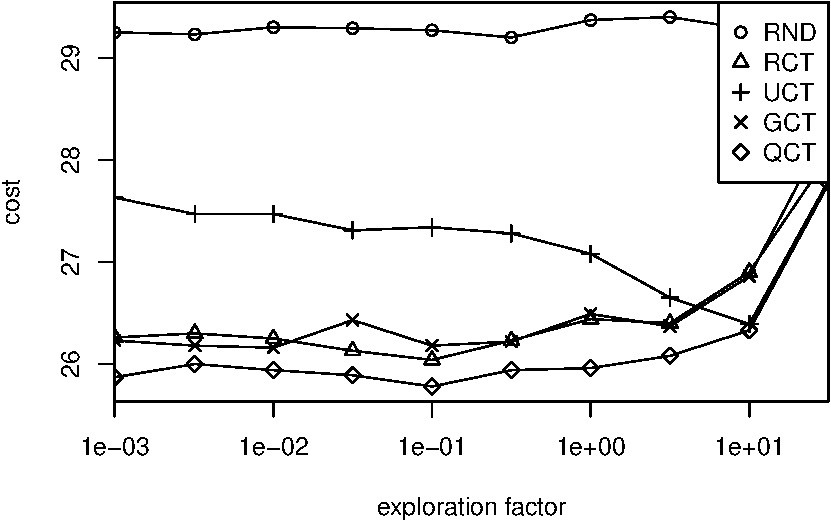
\includegraphics[scale=0.45]{costs-size=6-nsamples=397.pdf}\\
    b. 397 rollouts\\
  \end{minipage}
  \begin{minipage}[b]{0.5\linewidth}
    \centering
    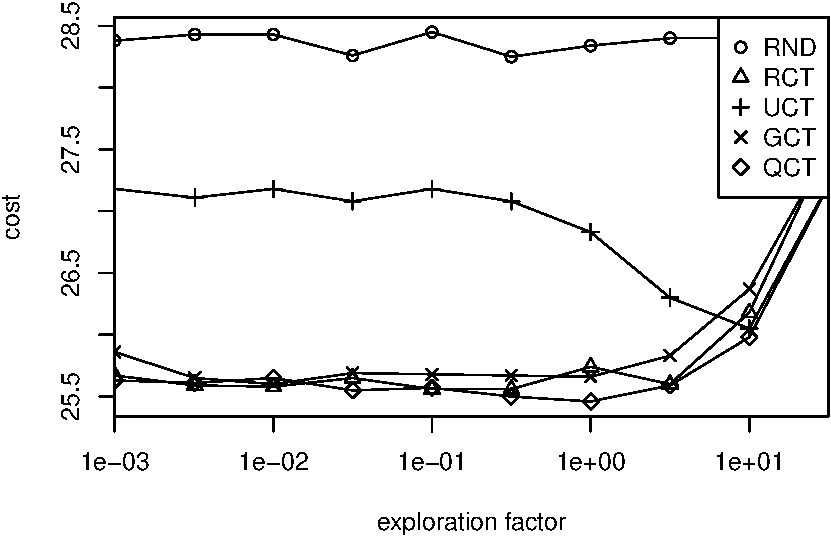
\includegraphics[scale=0.45]{costs-size=6-nsamples=793.pdf}\\
    c. 793 rollouts\\
    \vspace{1em}
    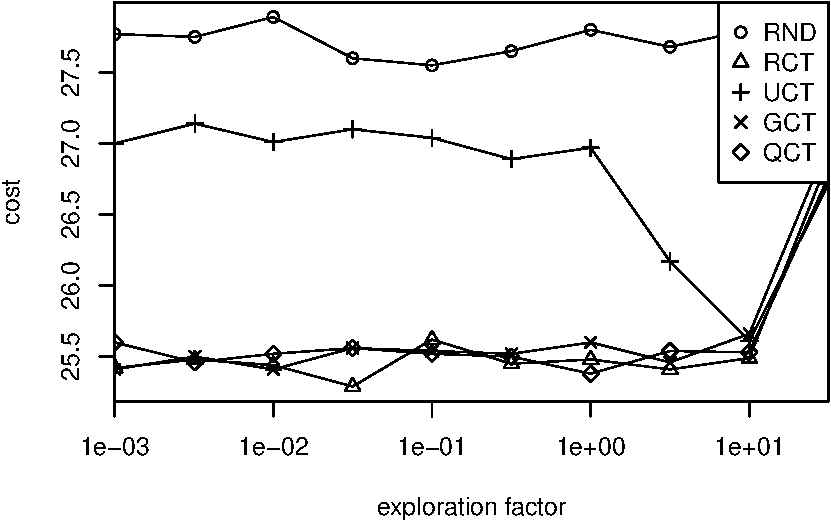
\includegraphics[scale=0.45]{costs-size=6-nsamples=1585.pdf}\\
    d. 1585 rollouts\\
  \end{minipage}
  \caption{The sailing domain, $6\times 6$ lake, cost vs. factor}
  \label{fig:sailing-cost-vs-factor}
\end{figure}


Figure~\ref{fig:sailing-lake-size} shows the cost vs. the exploration
factor for lakes of different sizes. The relative difference between
the sampling schemes becomes more prominent when the lake size
increases.

\begin{figure}[t]
  \begin{minipage}[b]{0.333\linewidth}
    \centering
    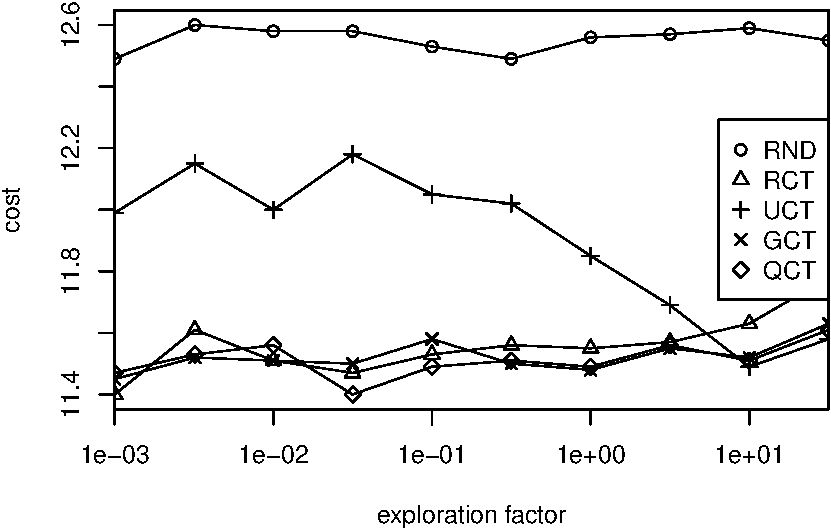
\includegraphics[scale=0.35]{costs-size=3-nsamples=397.pdf}\\
    a. $3\times 3$ lake
  \end{minipage}
  \begin{minipage}[b]{0.333\linewidth}
    \centering
    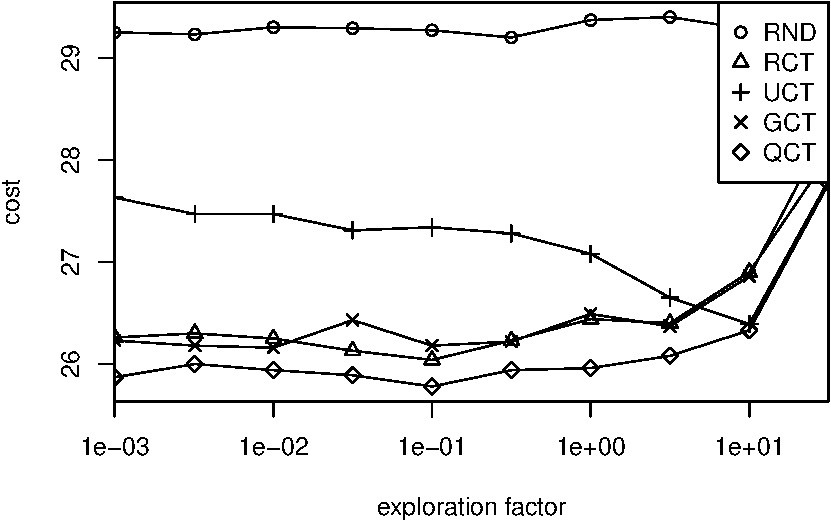
\includegraphics[scale=0.35]{costs-size=6-nsamples=397.pdf}\\
    b. $6\times 6$ lake
  \end{minipage}
  \begin{minipage}[b]{0.333\linewidth}
    \centering
    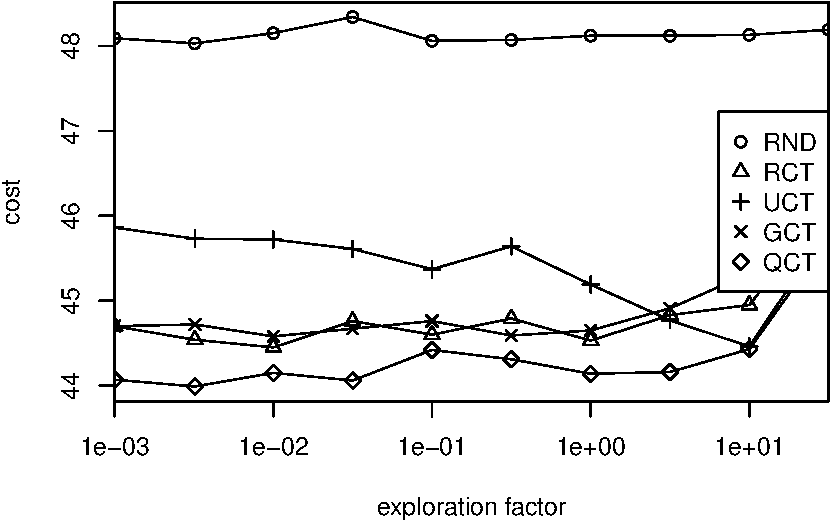
\includegraphics[scale=0.35]{costs-size=10-nsamples=397.pdf}\\
    b. $10\times 10$ lake
  \end{minipage}
  \caption{The sailing domain, 397 samples, cost vs. factor}
  \label{fig:sailing-lake-size}
\end{figure}

Figure~\ref{fig:sailing-rcq-vs-factor} compares QCT with UCT with a
different exploration factor at the root (CCT). $C_p$ for the rest of
the steps was chosen to ensure the best performance from earlier
experiments on the domain. Both algorithms exhibit similar dependency,
but as the number of samples grows, QCT achieves smaller average
regrets and is less sensitive to the choice of the value for $C_p$ at
the first step.

\begin{figure}[t]
  \begin{minipage}[b]{0.5\linewidth}
    \centering
    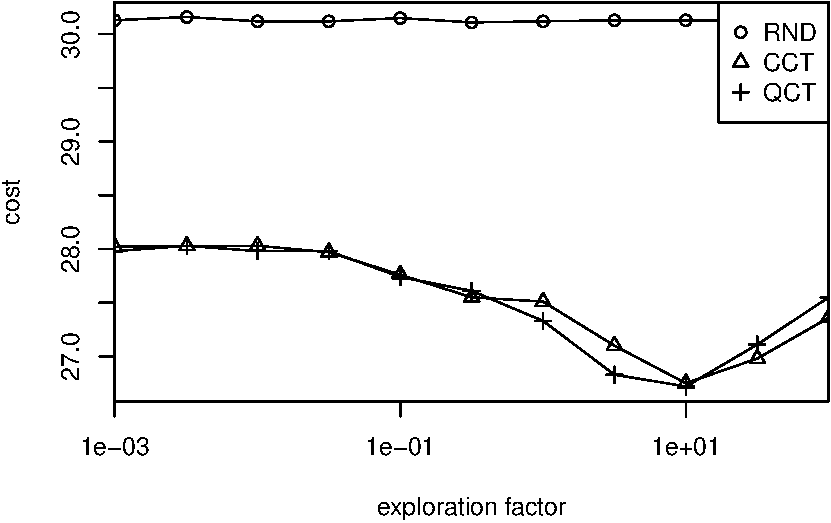
\includegraphics[scale=0.45]{rcq-size=6-nsamples=199.pdf}\\
    a. 199 rollouts\\
    \vspace{1em}
    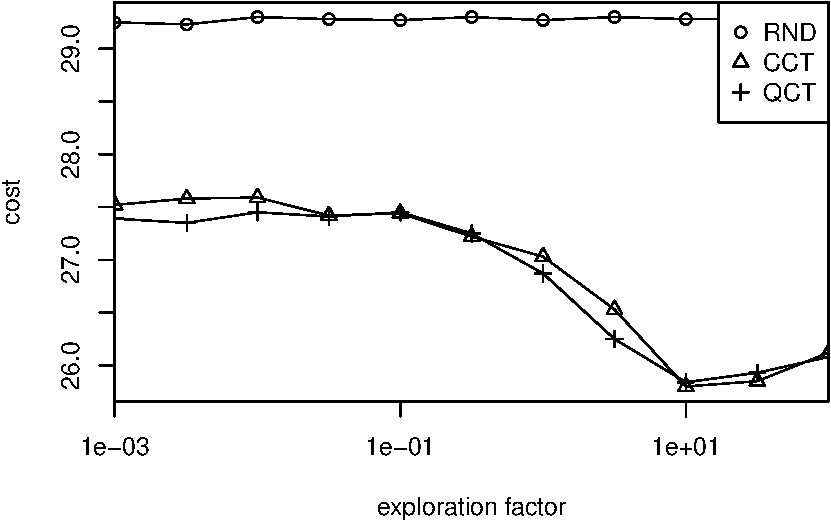
\includegraphics[scale=0.45]{rcq-size=6-nsamples=397.pdf}\\
    b. 397 rollouts\\
  \end{minipage}
  \begin{minipage}[b]{0.5\linewidth}
    \centering
    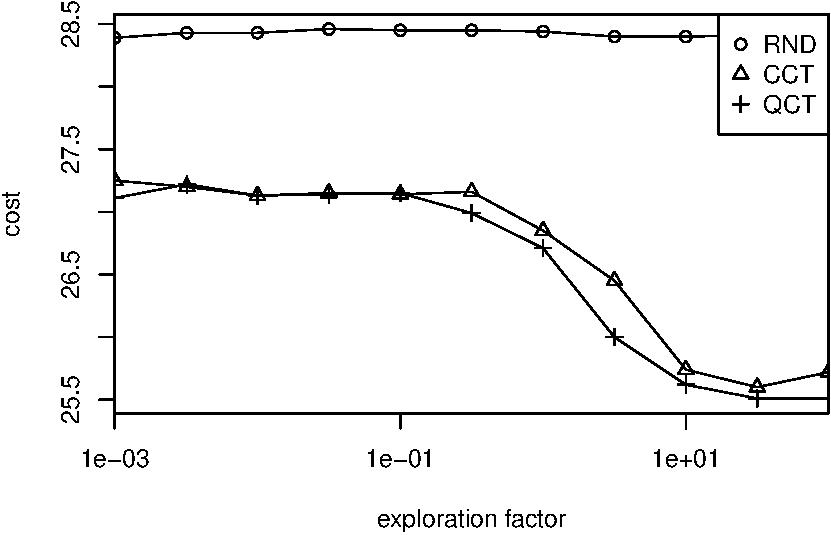
\includegraphics[scale=0.45]{rcq-size=6-nsamples=793.pdf}\\
    c. 793 rollouts\\
    \vspace{1em}
    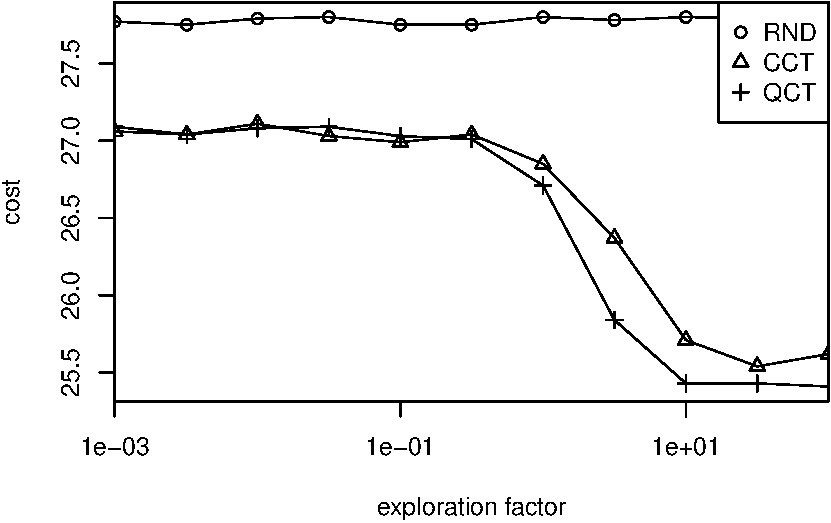
\includegraphics[scale=0.45]{rcq-size=6-nsamples=1585.pdf}\\
    d. 1585 rollouts\\
  \end{minipage}
  \caption{The sailing domain, log vs. sqrt, $6\times 6$ lake}
  \label{fig:sailing-rcq-vs-factor}
\end{figure}

\section{Summary and Future Work}

The Monte Carlo tree search algorithms presented in the paper differ
from UCT at the first step of the rollout, when the `simple' selection
regret is minimized instead of the cumulative regret. Both the
theoretical analysis and the empirical evaluation provide evidence for
better general performance of the proposed algorithms.

The improvement is inspired by the notion of value of information (VOI),
but VOI is used implicitly in the analysis of the algorithm, rather
than computed or learned explicitly in order to plan the rollouts. A
further improvement can be achieved by computing or estimating the VOI
of the rollouts and chosing a rollout that maximizes the VOI. Using VOI
to guide Monte Carlo sampling instead of relying on the sample means
of different actions  is particularly beneficial when different
actions have qualitatively different distributions: for example, when the
distribution variance varies signficantly between the actions.

\begin{figure}[t]
  \centering
  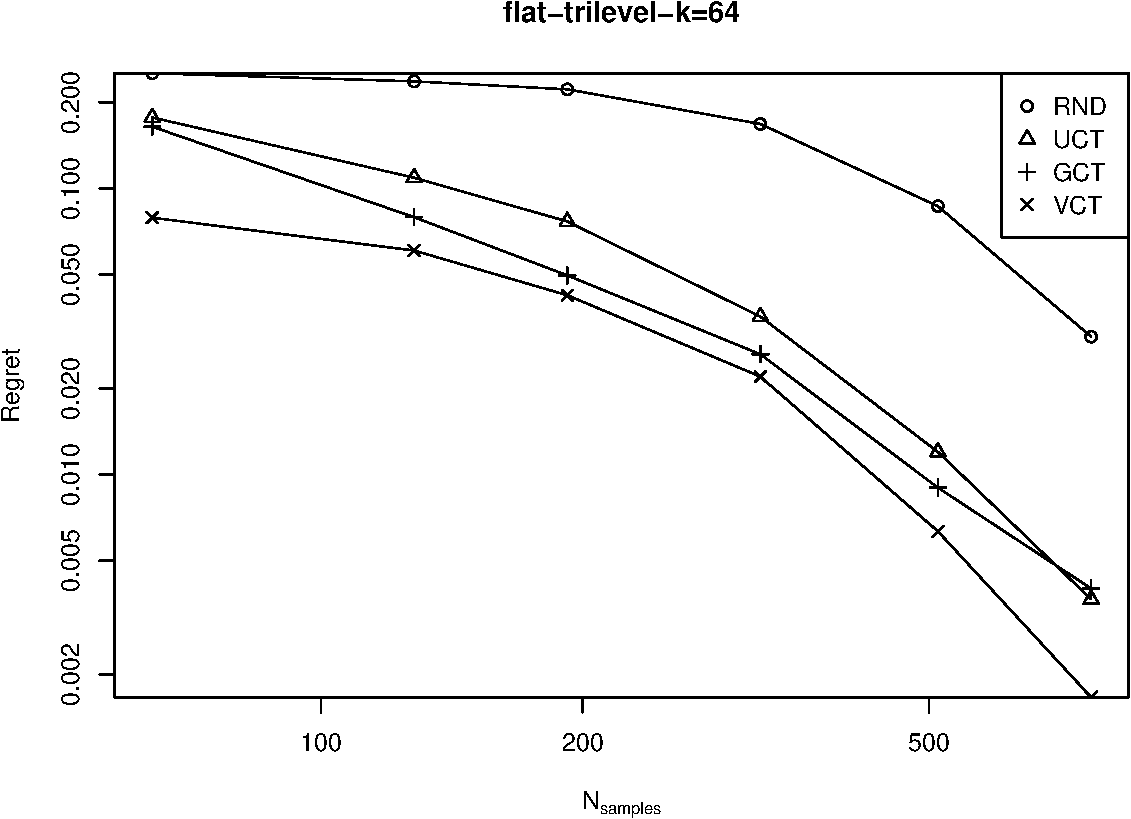
\includegraphics[scale=0.45,trim=0 0 0 16pt,clip]{flat-trilevel-vct-k=64.pdf}\\
  \caption{VOI-based action selection (VCT) vs. other algorithms}
  \label{fig:flat-trilevel-vct}
\end{figure}

VOI of a rollout can be computed when the sample distribution of an
action is known up to the parameters, such as the normal distribution
with an unknown mean and/or variance. Alternatively, the value of
information can be estimated from the set of samples, and the need to
assume a particular shape of the distribution is be lifted. In one
realization of the latter approach the VOI of performing an action is
estimated as \emph{the value of perfect information learned from the outcome
of earlier samples of the action divided by the number of
samples}. Early experiments with this approach showed the best
performance for sets of Bernoulli arms, and even a more prominent
improvement for mixed arms (e.g. Bernoulli, triangularly distributed,
and fixed arms) (Figure~\ref{fig:flat-trilevel-vct}):
\textbf{VCT}, the algorithm which selects an action with the maximum VOI estimate on
the first step exhibits lower average regret than other algorithms.
Sample-based VOI estimation requires keeping more information than an
algorithm based only on the sample
mean, but the overhead is small and
is justified by the improvement.

\section*{Acknowledgments}

The research is partially supported by Israel
Science Foundation grant 305/09, by the Lynne and William Frankel
Center for Computer Sciences, and by the Paul Ivanier Center for
Robotics Research and Production Management.

\clearpage
\appendix

\section{Facts}

{\bf Chernoff bounds (see \cite{Hagerup.chernoff}):} for $m$ independent random variables $X_1, X_2, ..., X_m$
taking on values 0 or 1, $X=\sum_{i=1}^m X_i$, and $0\le\delta\le 1$:
\begin{equation}
\Pr[X < (1-\delta)\IE[X]] < e^{-\delta^2\IE[X]/2} \mbox{ (Chernoff bound)}
\label{eq:chernoff-bound}
\end{equation}
Further on, if $\forall i. \IE[X_i]=\mu$:
\begin{equation}
\Pr[X < n\mu-a] <  e^{-2a^2/n}
\label{eq:chernoff-hoeffding-bound} \mbox{ (Hoeffding-Chernoff bound)}
\end{equation}

\section{Derivations}
\label{app:derivations}

\subsection{Finite-time regret bounds}
\label{app:derivations-finite}

%TODO: bounds on regret based on information gathered, independent of
%the way the choice is made.

For an analysis of pure exploration of uniform and UCB algorithms, see also
\cite{Bubeck.pure}.


\subsubsection{$\varepsilon$-greedy}
\label{app:derivations-finite-eps}

For $0<\varepsilon\le1-\frac 1 K$ and $x_0>0$ (see Section 3, Proofs, in \cite{Auer.ucb}):

\begin{eqnarray}
\Pr(\overline X_j=\max_i\overline X_i)&\le&2\left(x_0\cdot \Pr\left\{T_j^R(n)\le x_0\right\} + \frac 2{\Delta_j^2}e^{-\Delta_j^2\lfloor x_0 \rfloor/2}\right)\nonumber\\
&\le&2\left(x_0\cdot \Pr\left\{T_j^R(n)\le x_0\right\} + \frac {2 \cdot
  e^{\Delta_j^2/2}}{\Delta_j^2}e^{-\Delta_j^2 x_0 /2}\right)
\end{eqnarray}

Number of times $\xi$ the $j$th arm is selected {\it randomly}:

\begin{equation}
\xi\triangleq\IE\left[T_j^R(n)\right]=\frac {n\varepsilon} K
\end{equation}

By choosing $x_0=\frac \xi 2$ and applying the Chernoff bound (\ref{eq:chernoff-bound}), obtain:

\begin{eqnarray}
\label{eq:pr-epsilon-greedy}
\Pr(\overline X_j=\max_i\overline X_i)&\le& 2\left(\frac {\xi}{2} e^{-\xi/8} + \frac {2e^{\Delta_j^2/2}}{\Delta_j^2}e^{-\Delta_j^2 \xi/4}\right)\nonumber\\
&\le&\left(\xi + \frac {4\sqrt e}{\Delta_j^2}\right)e^{-\Delta_j^2\xi/8}
\end{eqnarray}

A bound on the simple regret $r_\varepsilon$ of an
$\varepsilon$-greedy policy follows from substituting
(\ref{eq:pr-epsilon-greedy}) into (\ref{eq:simple-regret}):

\begin{eqnarray}
  \IE r_\varepsilon&\le&\sum_{j=1}^K\Delta_j\left(\xi + \frac {4\sqrt e}
{\Delta_j^2}\right)e^{-\Delta_j^2\xi/8}\nonumber\\
&\le&K\left(\xi + \frac {4\sqrt
    e}{\Delta_{\min}}\right)e^{-\Delta_{\min}^2\xi/8}
\label{eq:deriv-epsilon-greedy-b}
\end{eqnarray}

\subsubsection{UCB($\alpha$)}
\label{app:derivations-finite-ucb}

$n_*$ pulls of the best arm and $n_j$ pulls of the $j$th arm are
achieved simultaneously when either 


\begin{equation}
\sqrt {\frac {\alpha \log n} {n_j-1}} \ge 1 + \sqrt { \frac {\alpha \log n} {n_*}}
\end{equation}

or

\begin{equation}
\sqrt {\frac {\alpha \log n} {n_j}} \le 1 + \sqrt { \frac {\alpha \log n} {n_* - 1}}
\label{eq:deriv-ucb-alpha-a}
\end{equation}

Inequality (\ref{eq:deriv-ucb-alpha-a}) can be used to derive a lower
bound on the number of pulls of a non-optimal arm,  and, consequently, the upper
bound on the probability of selecting a non-optimal arm:

\begin{eqnarray}
\frac {\alpha \log n} {n_j}&\le& 1 + 2  \sqrt {\frac {\alpha \log n}
  {n_*-1}} + \frac {\alpha \log n} {n_*-1}\nonumber\\
n_j &\ge& \frac {\alpha \log n} {1+2 \sqrt {\frac {\alpha \log n}
    {n_*-1}} + \frac {\alpha \log n} {n_*-1}}\nonumber\\
    &\ge& \frac {\alpha \log n} {4} \mbox{ for } \alpha \log n \le n_*-1
\end{eqnarray}

The probability that the $j$th arm will be chosen can be bounded using
the Chernoff-Hoeffding bound:
\begin{equation}
P_j \le 2 \exp\left(-\frac {\alpha \Delta_j^2 \log n} 8 \right) = 2n^{\frac {-\alpha \Delta_j^2} 8}
\end{equation}

The expected simple regret of an UCB($\alpha$) algorithm is thus
bounded by the following inequality:
\begin{equation}
\IE r_{ucb} \le 2\sum_{j=1}^K \Delta_jn^{\frac {-\alpha \Delta_j^2} 8}
\label{eq:deriv-ucb-alpha-b}
\end{equation}

\cite{Bubeck.pure} establishes for UCB($\alpha$) a similar bound,
polynomial in the number of pulls $n$.

\subsection{Asymptotic regret analysis}
\label{app:derivations-asym}

%TODO: Oracle instead of asymptotic

Bounds (\ref{eq:deriv-epsilon-greedy-b}, \ref{eq:deriv-ucb-alpha-b}) were
derived ignoring dependency of the allocation on expected values
of non-optimal arms. Derivation of better bounds seems
complicated. Instead, one can analyse the asymptotic behavior of each of the
algorithms under the assumption that the sample mean is close to the expectation.

\subsubsection{$\varepsilon$-greedy}
\label{app:derivations-asym-eps}


A common technique \cite{Auer.ucb} to bound the probability of
selecting a non-optimal arm $j$ is to split the interval between
$\mu_j$ and $\mu_*$ at the middle and bound the probability of
selecting the $j$th arm by the sum of the probabilities that the sample
mean $\overline X_j$ of the $j$th arm is greater than $\mu_j+\frac
{\Delta_j} 2$ and the sample mean $\overline X_*$ of the optimal arm is
less than $\mu_*- \frac {\Delta_j} 2$. Each of the probabilities can
be bound using the Chernoff-Hoefding bound.

Splitting the interval between $\mu_j$ and $\mu_*$ half-way is an
arbirtrary decision. By selecting a different split point
depending on the allocation of samples, one can obtain a tighter
bound. On the other hand, there is a value of $\varepsilon$ that
minimizes the bound for the $\varepsilon$-greedy allocation scheme.
Thus, the  $\varepsilon$-greedy allocation scheme can be tuned by
finding $\varepsilon$ that minimizes the bound obtained by
selecting the best split point. 

Split the interval $[\mu_j, \mu_*]$ at $\mu_j+\delta_j$. The
probability $P_j$ for selecting the
$j$th arm is bounded, using the union bound and the Chernoff-Hoeffding bound, as:

\begin{eqnarray}
P_j&\le&\Pr[\overline X_j>\mu_j+\delta_j]+\Pr[\overline X_*<\mu_*-(\Delta_j-\delta_j)]\nonumber\\
   &\le&\exp\left(-2\delta_j^2n_j\right)+\exp\left(-2(\Delta_j-\delta_j)^2n_*\right)
\end{eqnarray}

For the $\varepsilon$-greedy scheme, $n_i=\frac {\varepsilon n} K$,
$n_*=(1-\varepsilon)n$, thus

\begin{equation}
P_j \le \exp\left(-\frac {2\delta_j^2\varepsilon n} {K-1}\right) +\exp\left(-2(\Delta_j-\delta_j)^2(1-\varepsilon)n\right)
\end{equation}

In general, $\varepsilon$ and $\delta$ which minimize $P_j$ will
depend of $n$. For a constant $\varepsilon$, require that the
exponents in both terms are equal
\begin{eqnarray}
\exp\left(-\frac {2\delta_j^2\varepsilon n} {K-1}\right)
   &=& \exp\left(-2(\Delta_j-\delta_j)^2(1-\varepsilon)n\right)\\
\frac {\delta_j} {\Delta_j - \delta_j}
   &=& \sqrt { \frac {(K-1)(1-\varepsilon)} \varepsilon }
\label{eq:deriv-exps-equal}
\end{eqnarray}
and find conditional minima of $P_j(\delta_j, \epsilon)$ satisfying
either $\frac {\partial P_j} {\partial \delta_j}=0$ or $\frac {\partial P_j}
{\partial \varepsilon}=0$. 

\vspace{1em}
\paragraph{a. {\large $\frac {\partial P_j} {\partial \delta_j}=0$}}

\begin{eqnarray*}
\frac {4\delta_j\varepsilon n} {K-1}
  &-& 4(\Delta_j-\delta_j)(1-\varepsilon)n=0\\
\frac {\delta_j} {\Delta_j-\delta_j}&=&{ \frac {(K-1)(1-\varepsilon)} \varepsilon }
\end{eqnarray*}
and together with (\ref{eq:deriv-exps-equal}) this gives:
\begin{eqnarray}
\delta_j&=&\frac {\Delta_j} 2\nonumber\\
\varepsilon&=&1-\frac 1 K\nonumber\\
\IE r_{\varepsilon=1-1/K}&\le&B_{uniform}=2\exp\left(-\frac {\Delta_j^2n} {2K}\right)
\label{eq:deriv-uniform-sampling}
\end{eqnarray}

That is, the case $\frac {\partial P_j} {\partial \delta_j}=0$
corresponds to \emph{uniform random sampling}, and the tightest bound is obtained
by splitting the interval at the middle.


\paragraph{b. {\large $\frac {\partial P_j} {\partial \varepsilon}=0$}}

\begin{eqnarray*}
\frac {2\delta_j^2 n} {K-1}
  &-& 2(\Delta_j-\delta_j)^2n=0\\
\frac {\delta_j} {\Delta_j-\delta_j}&=&\sqrt {K-1}
\end{eqnarray*}
and together with (\ref{eq:deriv-exps-equal}) this gives:
\begin{eqnarray}
\frac {\delta_j} {\Delta_j}&=&\frac 1 {\sqrt {K-1}+1}\nonumber\\
\varepsilon&=&\frac 1 2\nonumber\\
\IE
r_{\varepsilon=1/2}&\le&B_{1/2\mbox{-}greedy}=2\exp\left(-\frac
  {\Delta_j^2n} {(\sqrt{K-1}+1)^2}\right)\nonumber\\
\lim_{K\to\infty}
\mathbb{B}r_{1/2\mbox{-}greedy}^K&=&2\exp\left(-{\Delta_j^2n}\right)\nonumber\\
\mbox{for large $K$: }\mathbb{B}r_{1/2\mbox{-}greedy}&\approx&2\exp\left(-\frac {\Delta_j^2n} K\right)
\label{eq:deriv-half-greedy-sampling}
\end{eqnarray}

That is, the case $\frac {\partial P_j} {\partial \varepsilon}=0$
corresponds to \emph{$\frac 1 2$-greedy sampling}, and for a large number of
arms $K$ 
\begin{equation}
\mathbb{B}r_{1/2\mbox{-}greedy}\approx \mathbb{B}r_{uniform}^2
\label{eq:derive-uniform-vs-half-greedy}
\end{equation}
Equation (\ref{eq:derive-uniform-vs-half-greedy}) suggests that
$\frac 1 2$-greedy sampling has a much higher convergence rate than uniform
sampling for a large number of arms.

\subsubsection{UCB($\alpha$)}
\label{app:derivations-asym-ucb}

The $UCB(\alpha)$ allocation scheme distributes arm pulls such that
the upper bound on the probability of selecting a non-optimal arm is
asymptotically the same for all arms. Indeed, for large n
\begin{eqnarray}
n_i&\ll&n\\
n_*&\approx&n\\
\sqrt {\frac {2 \log n} {n_j}}&\approx&\Delta_j+\sqrt {\frac {2\log n}
  {n_*}} \\
&\Rightarrow& n_j \approx \frac {2\log n} {\Delta_j^2}
\label{eq:deriv-ucb-asymptotic-nj}
\end{eqnarray}
and by Hoeffding-Chernoff bound the upper bound $\mathbb{B}P_j$ on the probability
$P_j^{ucb}$ to choose the $j$th arm is
\begin{equation}
P_j^{ucb}\le\mathbb{B}P_j^{ucb}\approx2\exp\left(-2\Delta_j^2\frac {2\log n}{\Delta_j^2}\right)
             =2n^{-4}
\end{equation}

That is, UCB($\alpha$) supposedly distributes pulls of non-optimal
arms better than $\varepsilon$-greedy
scheme which may undersample arms with high expectation. The
polynomial, rather than exponential, convergence rate (Equation
\ref{eq:deriv-ucb-alpha-b}) is due to oversampling the best arm.

Replacing the logarithm with a faster growing subpolynomial
function, like square root (UQB), results in a superpolynomial convergence
rate of the upper bound:
\begin{equation}
P_j^{uqb}\le\mathbb{B}P_j^{uqb}\approx2\exp\left(-\beta\Delta_j^2\frac {\sqrt n}{\Delta_j^2}\right)
            =2\exp(-\beta\sqrt n)
 \end{equation}
where $\beta$ is a constant that depends only on reward bounds.
Finite time convergence can still be shown similarly to UCB.


\bibliographystyle{plain}
\bibliography{refs}


\end{document}
